
%\documentclass[10pt,a4paper]{article}
\documentclass[runningheads]{llncs}
\usepackage[utf8]{inputenc}
\usepackage{amsmath}
\usepackage{amsfonts}
\usepackage{amssymb}


\usepackage{thmtools}
%\usepackage{amsthm}
\usepackage{thm-restate}
%\declaretheorem[name=Theorem,numberwithin=section]{thm}
%--experiment

\usepackage%[hidelinks]
			{hyperref}

\usepackage[capitalize, noabbrev]{cleveref}
\usepackage[autostyle=true]{csquotes}
\usepackage{graphicx}
\usepackage{color}
\usepackage{enumerate}
\usepackage{caption}
\usepackage{subcaption}


% Abstand obere Blattkante zur Kopfzeile ist 2.54cm - 15mm
%\setlength{\topmargin}{-15mm}


% Umgebungen für Definitionen, Sätze, usw.
% Es werden Sätze, Definitionen etc innerhalb einer Section mit
% 1.1, 1.2 etc durchnummeriert, ebenso die Gleichungen mit (1.1), (1.2) ..
%\newtheorem{theorem}{Theorem}[section]
%\newtheorem{definition}[theorem]{Definition} 
%\newtheorem{lemma}[theorem]{Lemma}
%\newtheorem{corollary}[theorem]{Corollary}	
%\newtheorem{example}[theorem]{Example}
%\newtheorem{observation}[theorem]{Observation}	
%\newtheorem{conjecture}[theorem]{Conjecture}
%\newtheorem{question}[theorem]{Question}			   
                  
\numberwithin{equation}{section}

\newcommand{\R}{\mathbb{R}}
\newcommand{\N}{\mathbb{N}}
\newcommand{\Z}{\mathbb{Z}}
\newcommand{\set}[1]{\{ #1 \}}
\newcommand{\fromto}[2]{\set{#1, \ldots, #2}}

\newcommand{\comment}[1]{\textcolor{red}{(L: #1)}}

\newcommand{\bigO}{\mathcal{O}}
\newcommand{\dotunion}{\mathbin{\dot{\cup}}}

\newcommand{\act}{\textsc{(Act)}}
\newcommand{\stact}{\textsc{(stAct)}}
\newcommand{\activation}{\textsc{Activation}}
\newcommand{\stactivation}{\textsc{st-Activation}}
\newcommand{\True}{\textsc{True}}
\newcommand{\False}{\textsc{False}}

\DeclareMathOperator{\ac}{\text{A}}
\DeclareMathOperator{\val}{\text{value}}
\newcommand{\vall}{w}
\DeclareMathOperator{\radius}{\text{radius}}

\DeclareMathOperator{\Nout}{N^\text{out}}
\DeclareMathOperator{\Nin}{N^\text{in}}
\DeclareMathOperator{\dom}{dom}
\DeclareMathOperator{\tw}{tw}
\DeclareMathOperator{\transhull}{trans-hull}
\DeclareMathOperator{\opt}{OPT}
\newcommand{\optAct}{\opt_\text{ACT}}
\newcommand{\optStAct}{\opt_\text{stACT}}
\newcommand{\optMenger}{\opt_\text{MENGER}}
\newcommand{\optSTP}{\opt_\text{STP}}
\newcommand{\optDirStAct}{\opt_\text{STACT}}
\newcommand{\optDirMenger}{\opt_\text{dir-MENGER}}
\newcommand{\optDirAct}{\opt_\text{dir-ACT}}
\newcommand{\optDirSTP}{\opt_\text{dir-STP}}


\begin{document}

\title{Keeping a network connected using nonpreemptive edge scheduling}
%
%\titlerunning{Abbreviated paper title}
% If the paper title is too long for the running head, you can set
% an abbreviated paper title here
%
\author{Stefan Lendl\inst{1} \and
Gerhard Woeginger\inst{2} \and
Lasse Wulf\inst{3}}
%
\authorrunning{S. Lendl, G. Woeginger, L. Wulf}
% First names are abbreviated in the running head.
% If there are more than two authors, 'et al.' is used.
%
\institute{
Department of Operations and Information Systems, University of Graz, Austria 
\email{stefan.lendl@uni-graz.at}\\
\and Department of Algorithmics and Complexity, RWTH Aachen, Germany 
\email{woeginger@algo.rwth-aachen.de}\\
\and Institute of Discrete Mathematics, Graz University of Technology, Austria\\
\email{wulf@math.tugraz.at}
}
%
\maketitle              % typeset the header of the contribution
%
\begin{abstract}
Consider the following process over time: Given a graph $G = (V,E)$ with positive integral edge weights $w$, we choose for each edge $e$ exactly one point in time $\tau_e \in [0, \infty)$. This causes $e$ to be active during $[\tau_e, \tau_e + w(e)]$. For (a) $F = V$ or (b) $F = \set{s,t}$, we introduce the problem of maximizing the time such that $F$ is connected by active edges. The problem is related to spanning tree packing, Menger's problem, and maximizing the minimum load time in nonpreemptive scheduling. We show that both (a) and (b) are NP-complete, even on instances with very restricted graph structure, or very restricted edge weights. For problem (a), we give some approximation results, and fixed-parameter-tractable results. For problem (b), we consider the relation to its relaxation, Menger's problem. 
\end{abstract}

\section{Introduction}
\comment{Comments by Lasse}
Suppose we have an electrical network, represented by a graph $G = (V,E)$, where each of the vertices represents a consumer or a producer, and each edge $e = \{u,v\}$ represents a power line between $u$ and $v$. However, the use of a power line $e$ is restricted by its \emph{weight} $w(e) \in \N$: We can only use it during an interval $[\tau_e, \tau_e + w(e)]$, where we may choose the \emph{activation time} $\tau_e \geq 0$ freely. In particular, we are not allowed to split this interval into multiple disjoint intervals of total length $w(e)$, i.e.\ the scheduling process is \emph{nonpreemptive}. We say that $e$ is \emph{active} during $[\tau_e, \tau_e + w(e)]$. In this paper, we consider two different problems:
\begin{enumerate}
\item \emph{Activation problem} \act: Keep the electrical network connected for as long as possible, i.e.\ choose the $\tau_e$ such that the subgraph of active edges is spanning for a maximal amount of time. 
\item \emph{s-t-Activation problem} \stact: Given $s, t \in V$, keep them connected for as long as possible, i.e.\ choose the $\tau_e$ such that $s, t$ are connected by active edges for a maximal amount of time.
\end{enumerate}

We stress the point that in general, at different points in time, the set of active edges is different. It is only required that at each point in time, the subgraph of active edges is spanning (is connecting $s$ and $t$). 

The problems \act\ and \stact\ are nonpreemptive variants of known problems. To see this, assume for a moment that we drop the condition of nonpreemptiveness, i.e.\ we allow activation of $e$ during multiple intervals, whose total length does not exceed $w(e)$. Then \stact\ becomes the problem of finding a maximum set of $s$-$t$-paths, such that for each edge, the number of paths crossing it does not exceed $w(e)$. This is called \emph{Menger's problem}. Similarily, the preemptive variant of \act\ is the problem of packing a maximum number of spanning trees into a weighted graph, i.e.\ the problem of \emph{spanning tree packing}. Both of these are classical problems and can be solved in strongly polynomial time. The first is solved by finding a maximal $s$-$t$-flow and finding a path decomposition of it, the second is solved either by matroid decomposition or flow techniques [cite]. There is a further connection to a classical problem from the area of job scheduling: The problem \act\ can be understood as a generalization of the problem of \emph{maximizing the minimum machine load time}. We can interprete this problem as an activation problem for uniform matroids, whereas problem \act\ is an activation problem for graphic matroids (details, see \cref{appendix:connection_act_job_scheduling}). Like both Menger's problem and spanning tree packing, this problem also has been considered extensively in the past [cite]. It is known to be strongly NP-complete, but to admit a PTAS [cite]. \comment{which exact papers should we cite for max-flow-min-cut, spanning tree packing, and maximizing min finish time?}

\emph{Our contribution.}
We introduce the problems \act\ and \stact. We show that \act\ is strongly NP-complete, even if a.) the input graph is $K_{2,n}$ or if b.) the input graph is outerplanar of bandwidth 2, or c.) we have $w(e) \in \fromto{1}{6}$. Furthermore, there is no fast (7/6)-approximation algorithm assuming P $\neq$ NP, even if $w(e) \in \fromto{1}{6}$. Similarily, we show that \stact\ is NP-complete, even if a.) the treewidth of the input graph is bounded by 3, or if b.) we have $w(e) \in \set{1,2}$ for all $e$. 
\cref{sec:positive_results} is concerned with positive results for {\act}. We give a linear time algorithm, if both the treewidth and edge weights are bounded by a constant. We describe an FPT-algorithm for the parameter of feedback edge set. We introduce a Greedy algorithm, which is a $(n-1)$-approximation. We show that the Greedy algorithm is optimal, if and only if the input graph is a cactus graph. Using techniques from extremal graph theory, we show in \cref{sec:ratio_relaxation}, that for problem \stact, the ratio to its relaxation, i.e.\ Menger's problem is unbounded.

\subsection{Definitions and Notation}
\label{sec_notation}

We write $\N_0 := \N \cup \set{0}$ for the set of nonnegative integers. For $a \leq b$, the term $[a, b]$ denotes the closed interval between $a$ and $b$. An instance for problem {\act} is a weighted, undirected graph $(G, w)$, where $G = (V, E)$ and $w : E \rightarrow \N$. We do not consider parallel edges. (However, it is easy to see that a pair of parallel edges can be easily modeled, by subdividing and using infinite or large enough edge weights.) A \emph{schedule} for some instance $(G, w)$ is simply a map $\sigma : E \rightarrow \N_0$, that maps each edge $e$ to its activation time $\sigma(e)$. 

Given a schedule $\sigma$ and an edge $e$, we denote the \emph{active interval of $e$} by $I_\sigma(e) := [\sigma(e), \sigma(e) + w(e)]$. We introduce discrete time steps: For $i \in \{1, 2, \dots\}$, the variable $E^\sigma_i := \set{e \in E : [i-1, i] \subseteq I_\sigma(e)}$ denotes the set of edges active in the $i$-th timestep, and the graph $G^\sigma_i := (V, E^\sigma_i)$ denotes the graph of active edges in the $i$-th timestep. For a vertex $v$, let $d^\sigma_i(v)$ denote the degree of $v$ in $G^\sigma_i$, i.e.\ the number of incident active edges of $v$ in the $i$-th timestep.
Let $C(\sigma) := \set{i \in \N : E_i^\sigma \text{ is spanning in } G^\sigma_i}$. The set $C(\sigma)$ is the set of all time steps, where the objective is fulfilled by the schedule $\sigma$. Finally, we define the \emph{value} of a schedule. If $C(\sigma) = \fromto{1}{T}$ for some $T$, let $\val(\sigma) = T$, else let $\val(\sigma) = 0$. When the schedule $\sigma$ is clear from the context, we also write $I(e), E_i$, $G_i$ and $d_i(v)$ instead of $I_\sigma(e), E^\sigma_i$, $G^\sigma_i$, and $d^\sigma_i(v)$. Using this new terminology, the problem {\act} is formally defined the following way:

\begin{quote}
Problem {\act}: 

\textbf{Input:} A tuple $(G, w)$ of a graph $G = (V,E)$ and positive integral edge weights.

\textbf{Output:} $\max\set{\val(\sigma) \mid \sigma \in (\N_0)^E}$.
\end{quote}

We give a short example of the introduced concepts. Consider the instance of problem {\act} depicted in \cref{fig:introduction_examples}. One has that the optimal value of a schedule is 2. A schedule $\sigma$ of value 3 does not exist, because in such a schedule there would be distinct edges $e, e'$ with $\sigma(e) = \sigma(e') = 0$. This implies $I(e) = I(e') = [0, 2]$, hence $G_3$ is not spanning. However, note that three spanning trees can be packed into this instance.
\begin{figure}
     \centering
         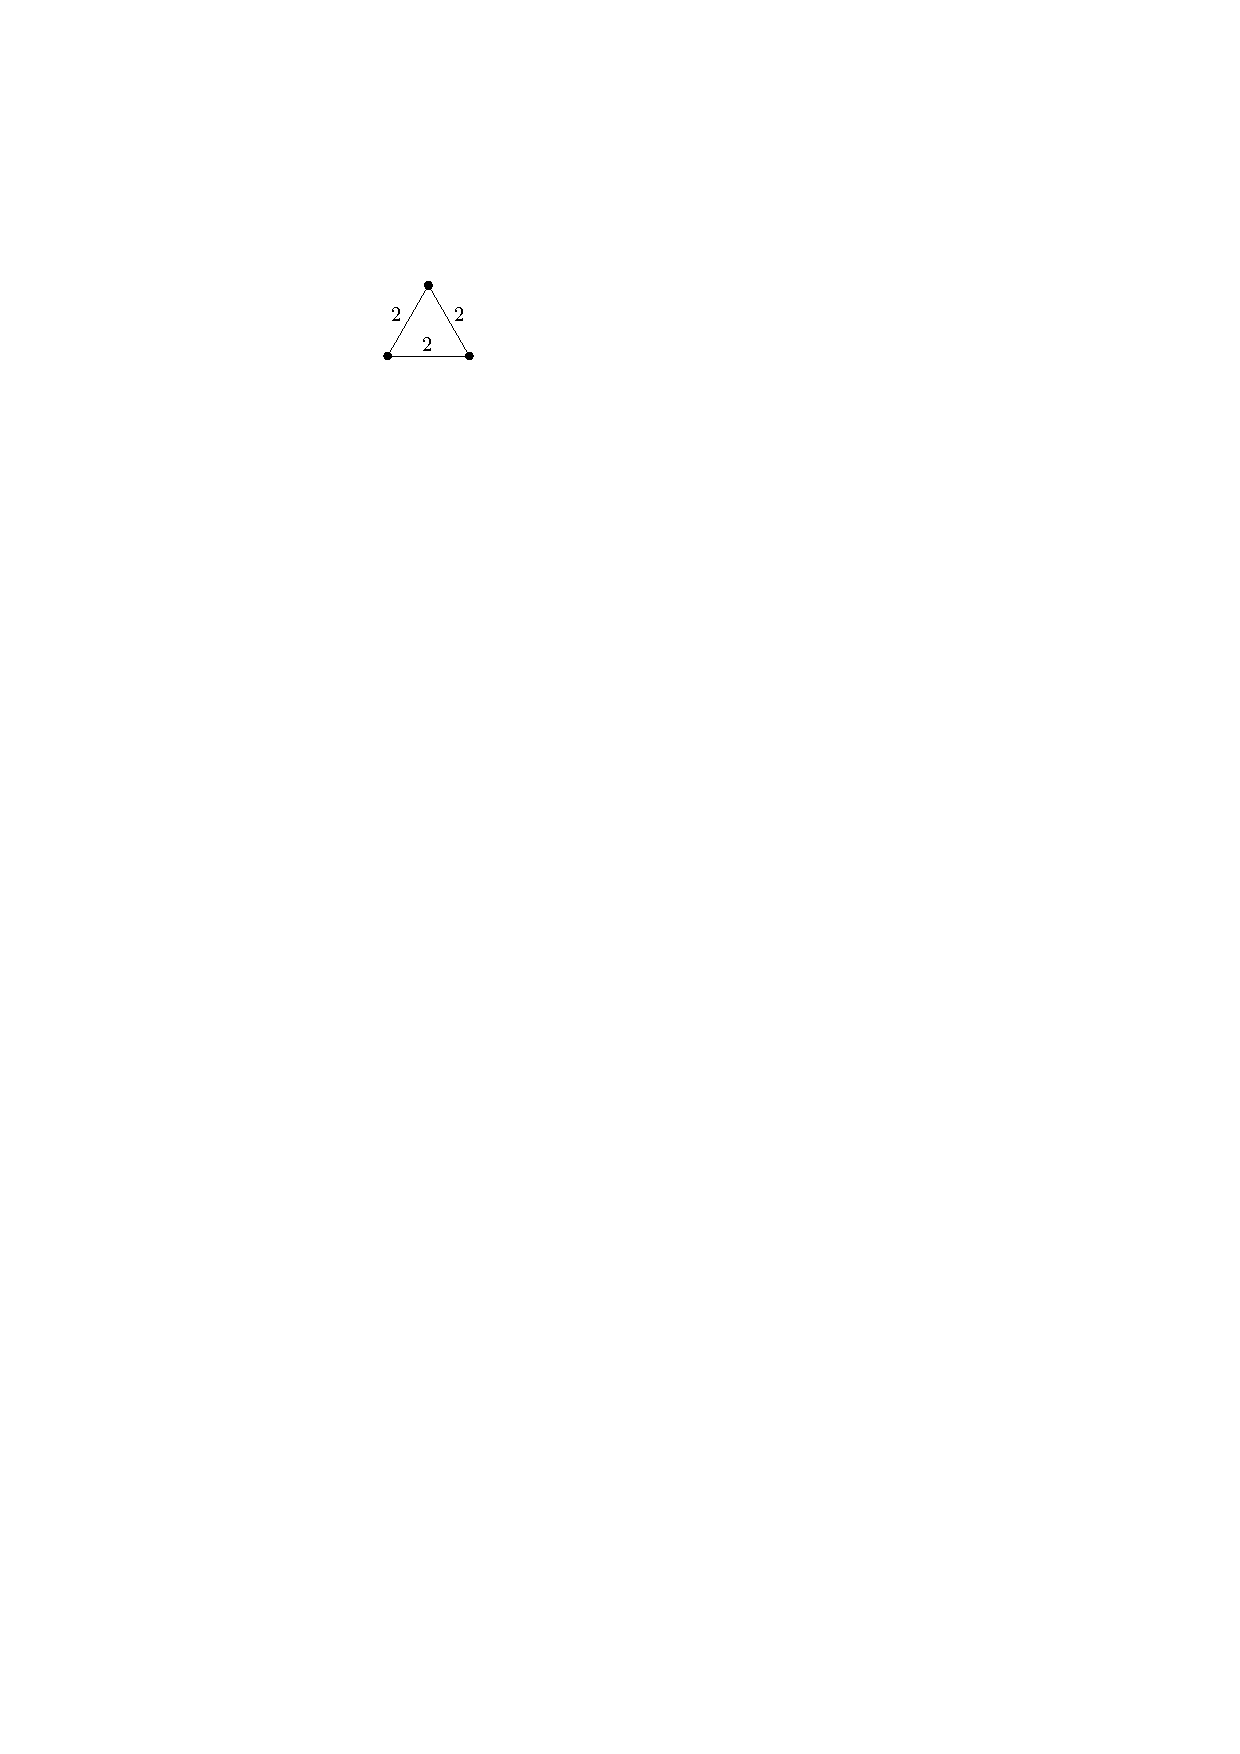
\includegraphics[scale=1]{img/example-act}
         \label{fig:example_act}
        \caption{Example instance for problem {\act}.}
        \label{fig:introduction_examples}
\end{figure}

We make use of the following graph-theoretic concepts and notations: Let $G = (V,E)$ be a graph. If $V' \subseteq V$ is a subset of the vertices, the corresponding \emph{edge cut} $\delta(V')$ is the set of edges having one endpoint in $V'$ and one endpoint in $V \setminus V'$. For a vertex $v$, we let $\delta(v) := \delta(\set{v})$. 
%If $(V_1,\dots,V_k)$ is a partition of $V$, the \emph{multicut} $\delta(V_1,\dots,V_k)$ is the set of edges with endpoints in diiferent parts of the partition. 
We denote by $G[V']$ the \emph{induced subgraph} on $V'$. By removing the vertex $v$ from $G$, we obtain $G - v := G[V \setminus \set{v}]$. Similarily, if $E' \subseteq E$ and $e \in E$, then $G - E' := (V, E \setminus E')$, and $G - e := G - \set{e}$.


\textbf{ Concepts currently used, but not defined: }
\begin{itemize}
\item definition path (i.e.\ no vertex twice, some call this specifically a simple path)
\item cactus graph
\item hamiltonian path/cycle
\item complete (bipartite) graph $K_n$, $K_{n,m}$
\item $\alpha$-approximation algorithm, Parameterized complexity, FPT-algorithm
\item Feedback edge set
\item treewidth
\item bandwidth
\item Monadic second-order graph logic $\text{MSO}_2$.
\end{itemize}

\section{NP-Hardness}
\label{sec:hardness}

In this section, we show NP-hardness of the problems {\act}, even if the input instances are restricted. 
This is done by reducing from the strongly NP-hard \textsc{3-Partition} problem~\cite{garey1979computers}: 


\begin{quote}

Problem \textsc{3-Partition}: Given a (multi-)set $A = \set{a_1, \ldots, a_{3n}} \subseteq \N$ with $Q/4 < a_i < Q/2$ for all $i$, where $Q := 1/n \sum A$, does there exist a partition of $A$ into $n$ into triplets, such that every triplet sums up to $Q$?

\end{quote}

In the following, we show that {\act} is strongly NP-hard for both series-parallel graph (see Theorem~\ref{thm:hardness_complete_bipartite}) and 
outerplanar graphs of bandwith~2 (see Theorem~\ref{thm:hardness_bandwidth}), both well studied families of 
graphs with treewdith~2.

\begin{theorem}
\label{thm:hardness_complete_bipartite}
The problem \act\ is strongly NP-complete if restricted to series-parallel graphs, even if the input graph is $K_{2,n}$.
\end{theorem}
\begin{proof}
Let $A = \fromto{a_1}{a_{3n}}$ be an instance of \textsc{3-Partition} and let $Q := 1/n \sum A$. Let $\beta := nQ + n - 1$. In order to prove NP-completeness, we construct an instance of problem \act\ with optimal objective value $\beta$, if and only if $A$ is a yes-instance of \textsc{3-Partition}. Consider the  complete bipartite graph $K_{2,4n-1}$ on the two vertex sets $\set{s, t}$ and $\set{x_1, \ldots, x_{n-1}, y_1, \ldots, y_{3n}}$. For $i \in \{1, \dots,n-1\}$, we set $w(\set{s,x_i}) := i(Q + 1)$ and $w(\set{x_i,t}) := (n - i)(Q + 1)$. For $i \in \{1,\dots,3n\}$, we set $w(\set{s,y_i}) := a_i$ and $w(\set{y_i,t}) := \beta$. 

Now, assume that for the described instance, there exists a schedule $\sigma$ of value $\beta$. Note that for all $i \in \{1,\dots,n-1\}$, we have $w(\set{s,x_i}) + w(\set{x_i,t}) = \beta + 1$, hence the sum of all weights is $(n-1)(\beta + 1) + 3n\beta + (\beta - n + 1) = \beta 4n$. Because the set of active edges is spanning at each point in time, and a spanning tree of $K_{2, 4n-1}$ has $4n$ edges, this implies that all of the graphs $G_1, \dots, G_\beta$ have exactly $4n$ edges and are spanning trees. 
For $i \in \{1,\dots,n-1\}$, consider the vertex $x_i$. Due to $w(\set{s,x_i}) + w(\set{x_i,t}) = \beta + 1$, there is exactly one $k \in [\beta]$, such that $d_k(x_i) = 2$. Furthermore, because the scheduling of the edges is nonpreemptive, and clearly $d_1(x_i) \geq 1$ and $d_\beta(x_i) \geq 1$, we can further deduce that $k$ has only the two possible values $i(Q+1)$ or $(n-i)(Q+1)$. Additionally, if there exists a $k$ such that for distinct $i, i' \in \{1,\dots,n-1\}$ one has $d_k(x_i) = d_k(x_{i'}) = 2$, then $G_k$ has a cycle, which is impossible. We conclude that there exists some $i \in \{1,\dots,n-1\}$ with $d_k(x_i) = 2$, if and only if $k \in \set{Q+1, 2(Q+1), \dots (n-1)(Q+1)}$. But this is a set of $n-1$ equidistant numbers, in $[\beta]$, such that $n$ gaps of size $Q$ are created. Using again acyclicity of $G_1, \dots, G_\beta$, it is easy to see that the scheduling of the edges $\fromto{\set{s,y_1}}{\set{s,y_{3n}}}$ implies a correct 3-partion of $A$.

On the other hand, assume $A$ is a yes-instance. Then it is easy to see that a schedule of value $\beta$ exists. (The schedule has the same properties as the schedule $\sigma$ in the first direction of the proof.)
\qed
\end{proof}

\begin{theorem}
\label{thm:hardness_bandwidth}
The problem \act\ is strongly NP-complete on outerplanar graphs of bandwidth 2.
\end{theorem}
\begin{proof}
Given an instance $A = \fromto{a_1}{a_{3n}}$ of \textsc{3-Partition} where $Q := 1/n \sum A$, we construct an instance of problem {\act}, whose optimal objective value is $\beta := (2n - 1)Q$, if and only if $A$ is a yes-instance of \textsc{3-Partition}.

The graph has $4n+1$ vertices $u_0,\ldots,u_n$ and $v_1,\ldots,v_{3n}$.
We will sometimes denote vertex $u_k$ also by the name $v_{k-n}$, for $1\le k\le n+1$;
in particular we use $u_n=v_0$ and $u_{n-1}=v_{-1}$.
\begin{itemize}
\item 
For $k=0,\ldots,n-1$,   the edge $\{u_k, u_{k+1}\}$ has weight $\vall(\{u_k, u_{k+1}\}) = 2(n-k-1)Q$.\\
For $k=0,\ldots,n-2$,   the edge $\{u_k, u_{k+2}\}$ has weight $\vall(\{u_k, u_{k+2}\})=2(k+1)Q$.
\item 
For $k=1,\ldots,3n$,    the edge $\{v_{k-1}, v_k\}$ has weight $\vall(\{v_{k-1}, v_k\})=a_k$.\\
For $k=-1,\ldots,3n-2$, the edge $\{v_k, v_{k+2}\}$ has weight $\vall(\{v_k, v_{k+2}\})=\beta$.  
\end{itemize}
In the ordering $u_0,u_1,\ldots,u_n,v_1,v_2,\ldots,v_{3n}$, every edge either connects two neighboring 
vertices or two vertices at distance~$2$. Hence, the constructed graph $G=(V,E)$ has bandwidth~$2$. 
This implies that $G$ furthermore is outerplanar.

We will study schedules $\sigma$ of value $\beta$. Notice that the sum of all weights in $G$ equals $\beta(|V| - 1)$. Hence, if $\sigma$ is such a schedule of value $\beta$, then each of $G^\sigma_1, \dots G^\sigma_\beta$ is a spanning tree and acyclic.

In particular, we will consider the behavior of $\sigma$ on the induced subgraph $H_i := G[\fromto{u_0}{u_i}]$ for $1\le i\le n$.
Since the only connections between $H_i$ and the rest of the graph are via the two vertices $u_{i-1}$ and $u_i$,
at any moment $t\in [0,\beta]$ in time, graph $H_i$ will consist of one or two connected components
under schedule $\sigma$.
If there is a single connected component, we say that $H_i$ is \emph{fully-connected} at time $t$.
If there are two connected components (one containing vertex $u_{i-1}$, the other one containing 
vertex $u_i$), we say that $H_i$ is \emph{semi-connected} at time $t$.
Note that if $H_i$ is semi-connected at moment $t$, then the edge $\{u_{i-1}, u_{i+1}\}$ must be active at 
that moment $t$, as there are no other edges that would be able to connect the component containing 
$u_{i-1}$ to the rest of the graph.

The graph $H_1$ consists of the vertices $u_0$ and $u_1$ and of the edge $\{u_0, u_1\}$ of weight $(2n-2)Q$.
Suppose for the sake of contradiction that $H_1$ is neither fully-connnected at $t=0$ nor at $t=\beta$:
Then the edge $\{u_0, u_2\}$ (of value $2Q$) must be active at $t=0$ and at $t=\beta$, which is impossible.
By symmetry, we will henceforth assume that under schedule $\sigma$ the graph $G_1$ is fully-connnected at $t=\beta$.
This implies that $\{u_0, u_1\}$ is active during $[Q,\beta]$ and that $\{u_0, u_2\}$ is active during $[0,2Q]$.
For graph $H_i$ (with $1\le i\le n$) one can show by induction that $H_i$ is semi-connected
during the time intervals $[0,Q]$, $[2Q,3Q]$, \dots, $[(2i-2)Q,(2i-1)Q]$ and fully-connected at all
other moments in $[0,\beta]$.
The induction uses the following facts and observations on the two edges $\set{u_{i-2}, u_i}$ and $\set{u_{i-1},u_i}$ 
that are in $H_i$ but not in $H_{i-1}$:
\begin{itemize}
\item Graph $H_i$ is semi-connected at time $0$. (This is because we have by induction hypothesis that $H_{i-1}$ is semi-connected at $t=0$, so if $H_i$ would be fully-connected at $t=0$, this would imply $\sigma(\{u_{i-2}, u_i\}) = \sigma(\{u_{i-1}, u_i\}) = 0$. But then, because all involved edges have weight $w(e) > Q$, at time $t = Q+1$ we have a cycle, which is impossible.)
\item Since $H_{i-1}$ is semi-connected at time $0$, the edge $\{u_{i-2},u_i\}$ must be active at time $0$
and hence must be active during $[0,(2i-2)Q]$.
\item $H_i$ must be fully-connnected at time $\beta$. (Otherwise, $H_i$ is fully-connnected neither 
at $t=0$ nor at $t=\beta$, and the edge $\{u_{i-1},u_{i+1}\}$ had to be active for $\beta$ time units.)
\item Since $H_i$ is fully-connnected at time $\beta$, the edge $\{u_{i-1},u_i\}$ must be active at time $\beta$
and hence must be active during $[(2i-1)Q,\beta]$.
\end{itemize}
The induction yields for $i=n$ that the induced subgraph $H_n$ is semi-connected during the time intervals 
$[0,Q]$, $[2Q,3Q]$, \dots, $[(2r-2)Q,(2r-1)Q]$ (that is, all the intervals of length $Q$ that start at an even multiple of $Q$)
and fully-connected during the time intervals $[Q,2Q]$, $[3Q,4Q]$, \dots, $[(2n-3)Q,(2n-2)Q]$ (that is, all the 
intervals of length $Q$ that start at an odd time multiple of $Q$).

Next, consider the subgraph $G'$ that is induced by the $3n+2$ vertices $v_{-1}=u_{n-1}$, $v_0=u_n$ and 
$v_1,\ldots,v_{3n}$.
As the edges $\{v_k, v_{k+2}\}$ with $k=-1,\ldots,3n-2$ all have value $\beta$, there is an active path $P_0$ 
through the vertices with even index during the full interval $[0,\beta]$ and there is an active 
path $P_1$ through the vertices with odd index during $[0, \beta]$.
By the above discussion, graph $H_n$ connects these two paths $P_0$ and $P_1$ to each other during the
time intervals $[Q,2Q]$, $[3Q,Q4]$, \dots, $[(2n-3)Q,(2n-2)Q]$.
The only way for connecting $P_0$ and $P_1$ to each other during the remaining time intervals 
$[0,Q]$, $[2Q,3Q]$, \dots, $[(2n-2)Q,(2n-1)Q]$ is by using the edges $\{v_{k-1},v_k\}$ with $k=1,\ldots,3n$ of 
weight $a_k$.
As this groups the numbers $a_1,\ldots,a_{3n}$ into $n$ groups with sum $Q$, we get a solution
for the instance of \textsc{3-Partition}.
Vice versa, if the \textsc{3-Partition} instance has a solution, then we can build a schedule $\sigma$
with all desired properties from it.
\end{proof}

\section{Hardness of Approximation}
\label{sec:inapprox}

\cref{thm:hardness_complete_bipartite,thm:hardness_bandwidth} show NP-hardness, even if the structure of the input graph is heavily restriced. 
We now show that assuming $P \neq NP$ there exists no $\alpha$-approximation algorithm for problem {\act}, for 
any $\alpha < 7/6$, even if $w(e) \in \{1,\dots,6\}$.
%We now show hardness even if the weights $w(e)$ are restricted. 
For this, we reduce from the Hamilton cycle problem. Akiyama, Nishizeki and Saito proved that the Hamilton cycle problem is NP-complete even for bipartite, 3-regular graphs \cite{hamilton3regularBip}. We additionally require hardness for a more restricted variant of the hamilton cycle problem, which we call \textsc{Hamilton'}. NP-completeness of \textsc{Hamilton'} is surely known, however, we were unable to find it in the literature. We give a proof in \cref{appendix:hamilton_prime}.

\begin{quote}

Problem \textsc{Hamilton'} 

\textbf{Given:} An undirected, bipartite and 4-regular graph $H$, a special edge $\set{u, z}$, such that the following three are equivalent: (i) $H$ has a Hamilton cycle; (ii) $H$ has a Hamilton cycle using the edge $\set{u, z}$; (iii) $H$ has a Hamilton path starting at $u$.

\textbf{Question:} Does there exist a Hamilton cycle in $H$?

\end{quote}

\begin{restatable}{lemma}{hamiltonPrime}
\label{hamilton_cycle_lemma}
\textsc{Hamilton'} is NP-complete.
\end{restatable} 

Using the above lemma, we can construct a gap reduction to show:

\begin{theorem}
\label{corollary_act_no_approx}
%The problem {\act} is NP-complete, even if $w(e) \in \fromto{1}{6}$ for all edges. Furthermore, if $P \neq NP$, there is no poly-time $\alpha$-approximation with $\alpha < 7/6$, even if $w(e) \in \fromto{1}{6}$ for all edges.
If $P \neq NP$, there is no poly-time $\alpha$-approximation with $\alpha < 7/6$ for problem {\act}, even if $w(e) \in \fromto{1}{6}$ for all edges.
\end{theorem}
\begin{proof}
Let $H$ be an instance of the problem \textsc{Hamilton'}. We construct in polynomial time an instance $(G, w)$ of problem {\act}, such that $w(e) \in \fromto{1}{6}$ for all edges, and such that the optimal value of a schedule is at most 7, and is equal to seven if and only if $H$ has a Hamilton cycle. This is sufficient to prove the theorem.

The reduction is depicted in \cref{fig_act_hamilton_cycle}. Let the two bipartite parts of $H$ be $U = \fromto{u_1}{u_k}$ and $Z = \fromto{z_1}{z_k}$, and let $\set{u_k, z_k} =: e_0$ be the special edge of the given \textsc{Hamilton'} instance. The graph $G$ consists of a copy of $H$ where every edge has weight 2, except $e_0$, which has weight 1. Furthermore, there is an additional vertex $x$, which is connected to each of $\fromto{u_1}{u_k}$ via the gadget $L$ and to each of $\fromto{z_1}{z_k}$ via the gadget $R$. Finally, there is an additional vertex $y$ connected to both $x$ and $y$ with an edge of weight 4.
\begin{figure}[htpb]
     \centering
     \begin{subfigure}[b]{0.4\textwidth}
         \centering
         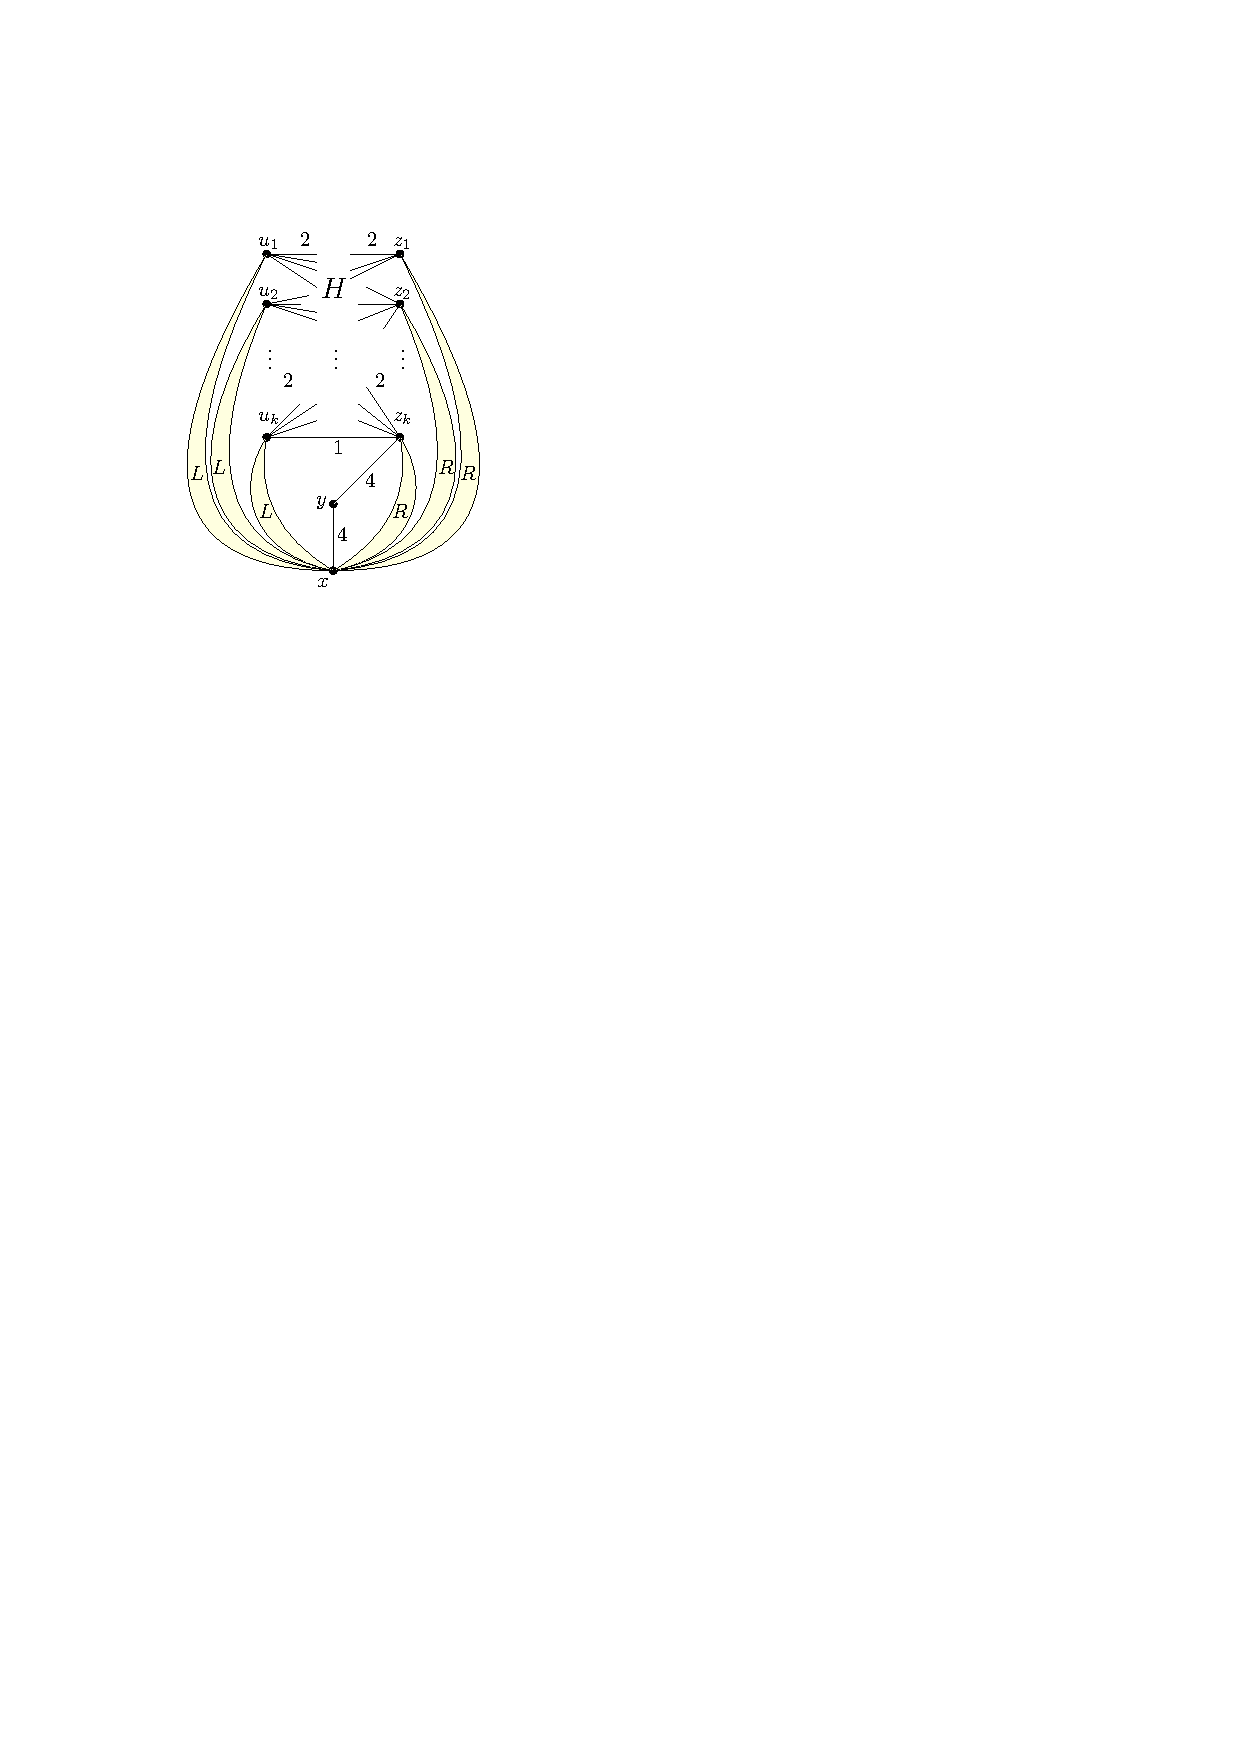
\includegraphics[scale=1]{img/act-hamilton-cycle-a}
         \subcaption{Reduction}
     \end{subfigure}
     \hfill
     \begin{subfigure}[b]{0.3\textwidth}
         \centering
         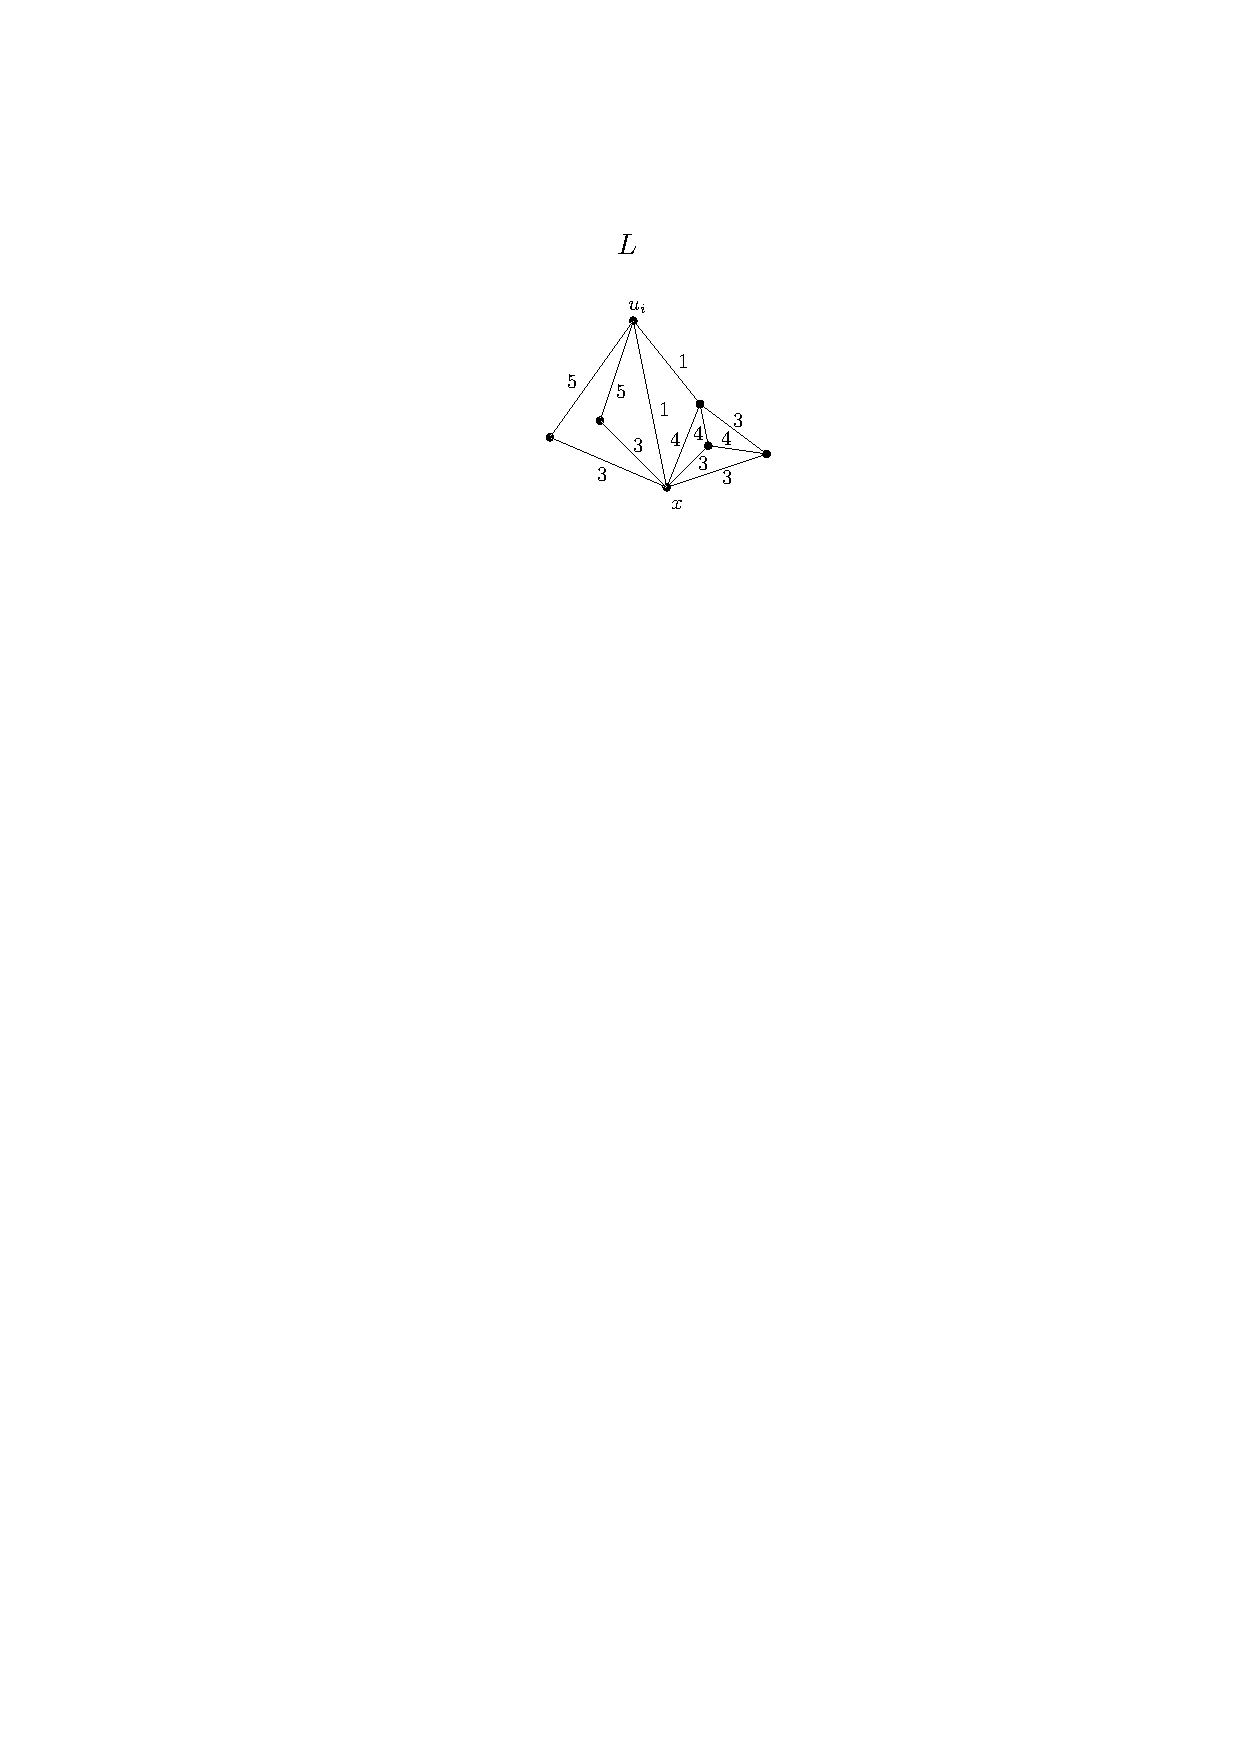
\includegraphics[scale=1]{img/act-hamilton-cycle-b}
         \subcaption{Gadget $L$}
     \end{subfigure}
     \hfill
     \begin{subfigure}[b]{0.15\textwidth}
         \centering
         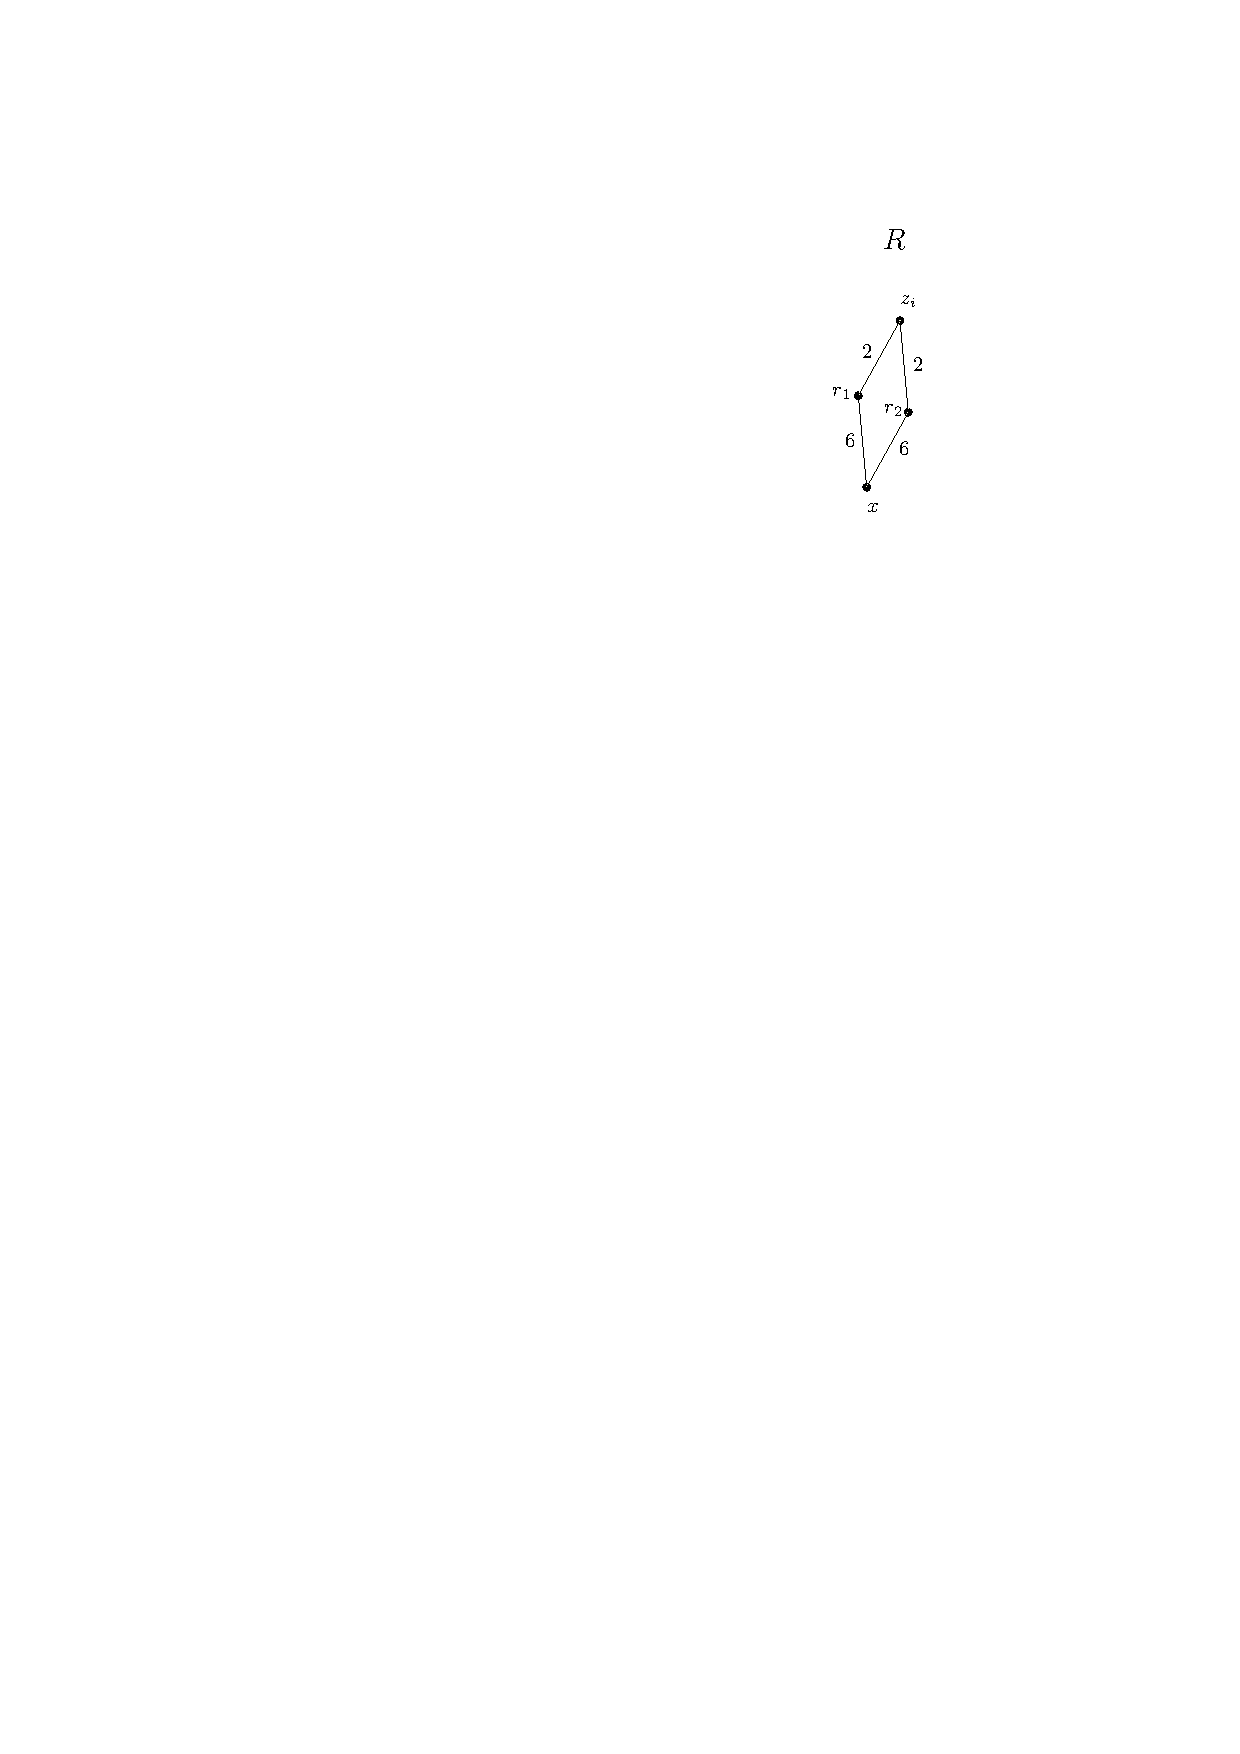
\includegraphics[scale=1]{img/act-hamilton-cycle-c}
         \subcaption{Gadget $R$}
     \end{subfigure}
        \caption{Reduction \textsc{Hamilton'} $\rightarrow$ {\act}.}
        \label{fig_act_hamilton_cycle}
\end{figure}

We first describe the properties of the gadgets $L$ and $R$. Assume $\sigma$ is a schedule of value 7. Note that the sum of all weights in $G$ is $8k - 1 + 39k + 16k + 8 = 63k + 7 = 7(|V(G) - 1|)$. Therefore, each of $G_{1}, \ldots, G_{7}$ is a tree, and in particular acyclic. By inspecting the vertices $r_1$ and $r_2$ and using acyclity of $G_2, G_6$ we see that the gadget $R$ necessarily connects $x$ and $z_i$ in $G_2$ and $G_6$, but does not connect $x$ and $z_i$ in $G_t$ for $t \neq 2,6$. Similarily, the gadget $L$ necessarily connects $x$ and $u_i$ in $G_3$ and $G_5$ and has some remaining edges, which are not restricted and behave like two parallel edges of weight 1. Analogously, $G_{t}[\set{x, y, w_k}]$ is connected if and only if $t = 4$.

Now, suppose $H$ is a yes-instance of \textsc{Hamilton'}, i.e.\ $H$ has a Hamilton cycle $C$, which contains $e_0$. Then $H - E(C)$ is 2-regular, hence there exist pairwise disjoint matchings $M_1, \ldots, M_4$ such that $M_1 \dotunion M_2 = E(C)$ and $M_3 \dotunion M_4 = E(H) \setminus E(C)$ and $e_0 \in M_1$. Consider the following schedule: We schedule $e_0$ in $G_3$; $M_1 \setminus \set{e_0}$ in both $G_3$ and $G_4$; $M_2$ in both $G_4$ and $G_5$; $M_3$ in both $G_1, G_2$; and $M_4$ in both $G_6$ and $G_7$. We schedule the gadgets such that $U$ is connected to $x$ via the $L$'s in $G_1, G_3, G_5$ and $G_7$, and that $Z$ is connected to $x$ via $R$'s in $G_2$ and $G_6$, and that $x$ is connected to $z_k$ via $y$ in $G_4$. Now observe that the active edges in $U \cup Z$ form a matching of $H$ in $G_1, G_2, G_3, G_5, G_6$ and $G_7$ and a Hamiltonian path in $G_4$. It is easy to see that this is a valid schedule of value 7. 

On the other hand, suppose there exists a schedule $\sigma$ of value 7 for $(G, w)$.
Recall the properties of the gadgets $L$ and $R$. Then, for $t' \in \set{1, 7}$, consider $G_{t'}$ and some $z_i$ for $i \in \fromto{1}{k-1}$. Note that for all $t \in \set{1, 3, 4, 5, 7}$ at least one of the edges in $\delta(z_i) \cap E(H)$ is active. This implies that $z_i$ has degree equal to 1 in $G_{t'}[U \cup W]$, due to the different possibilities of covering the set $[0, 1] \cup [2, 5] \cup [6, 7]$ with 4 intervals of length 2. Similarly, by considering $t' \in \set{1, 7}$, and $t \in \set{1, 3, 5, 7}$, we see that $z_k$ has degree equal to 1 in $G_{t'}[U \cup W]$ and that $e_0 \not \in E(G_{4})$. So all $z \in Z$ have degree 1 in $G_{t'}[U \cup H]$. But this implies that $G_{t'}[L']$ is connected for each copy $L'$ of $L$, otherwise $U$ is disonnected in $G_{t'}$. Hence $G_t[L']$ is connected if and only if $t \in \set{1, 3, 5, 7}$. Hence, for $u \in U$ and $t' \in \set{2, 6}$, we have that the degree of $u$ in $G_{t'}[U \cup W]$ is at least one. Consider the graph $F := G_{4}[U \cup Z]$: Due to the lower bound of the minimum degrees for $t' \in \set{1, 7}$ or $t' \in \set{2, 6}$, we have that the maximum degree in $F$ is two. We claim that the degree of $u_k$ in $F$ is equal to 1. In fact, assume the opposite and consider $u_k$. We know that $e_0 \not\in E(G_4)$, so the edges adjacent to $u_k$ scheduled in $G_4$ are not $e_0$. But $u_k$ has only four adjacent edges in $H$, and we have a requirement on the minimum degree of $u_k$ for $t' \in \set{2, 6}$. We conclude $e_0 \in E(G_2)$ or $e_0 \in E(G_6)$. But now consider $z_k$. We have a requirement on the minimum degree for $t' \in \set{1, 3, 5, 7}$. Because $e_0 \in E(G_2) \cup E(G_4)$ and $w(e_0) = 1$, this is requirement is impossible to fulfill.
In summary, $F$ is a graph of maximum degree 2, where $u_k$ has degree 1. It follows from the state of the gadgets in $G_4$, that $F$ is connected. We conclude that $F$ is a Hamiltonian path in $H$ starting at $u_k$. Therefore $H$ is a yes-instance of \textsc{Hamilton'}.

%%Due to the different possibilities of covering the interval $[0, 7]$ with four intervals of length 2, we have that for $t' \in \set{0.5, 6.5}$, each of $w_1, \ldots w_{k-1}$ has degree 1 in $G_{t'}$. Similarly, both $y, w_k$ have degree 1 in $G_{t'}$. We conclude that $u_1, \ldots, u_k$ lie in $k$ different connected components of $G_{t'} - x$ and hence $G_{t'}$ has an edge connecting $x$ and $u_i$ for each $i$. But then, $G_{3.5}$ has none of the edges between $x$ and $u_i$, hence $G_{3.5}[Z]$ is connected, where $Z := \set{u_1, \ldots, u_k, w_1, \ldots, w_k}$.  Again, by the different possibilities of covering the interval $[0, 7]$ with subintervals, we conclude that in $G_{3.5}$, the vertices $u_k, w_k$ have degree 1, $e_0 \not\in E(G_{3.5})$, and each of $w_1, \ldots w_{k-1}$ have degree at most two. They also have degree exactly two, otherwise we find a cyle in one of $\set{G_{0.5}, \ldots, G_{6.5}} \setminus \set{G_{3.5}}$. 
\end{proof}


\section{Positive Results}
\label{sec:positive_results}

In this section, we present exact solution approaches for restricted instances, and approximation results for problem {\act}. Unfortunately, the arguments presented here do not generalize to \stact. It is an open question to find similar results for \stact. 

\subsection{FPT-algorithms}

\begin{theorem}
If both the treewidth and the maximum edge weight $w(e)$ of an instance are bounded by  a constant $k$, problem {\act} can be solved in linear time. (There is an FPT-algorithm with respect to $k$). 
\end{theorem}
\begin{proof}
Let $(G, w)$ be an instance of {\act}, such that $G = (V, E)$ has treewidth at most $k$, and $w(e) \leq k$ for all edges. Because $G$ has treewidth at most $k$, there exists a vertex $v$ of degree at most $k$. Every edge incident to $v$ has weight at most $k$. Hence the maximum value of a solution is at most $k^2$. For every $T \in [k^2]$, we construct a formula $\Phi_T$ in monadic second-order graph logic $\text{MSO}_2$, such that $\Phi_T$ is satisfiable if and only if a schedule of value $T$ exists. In fact, we introduce binary variables $x_{e,t}$ for $e \in E$ and $t \in [T]$. Then the following expression can be formulated in $\text{MSO}_2$:
\begin{align*}
\exists \sigma :  E \rightarrow \fromto{0}{T} : &\forall e \in E, t \in [T]: (x_{e,t}=1) \leftrightarrow \left(\sigma(e) < t \leq \sigma(e) + w(e)\right)\\
\land &\forall t \in [T]: \set{e \in E \mid x_{e,t} = 1} \text{ is spanning.}
\end{align*}
It follows from Courcelle's theorem \cite{courcelle1990monadic}, that for each $T \in [k^2]$, the satisfiability of $\Phi_T$ can be checked in linear time. This proves the claim.
\end{proof}

\begin{theorem}
For instances $(G, w)$ without any restrictions on the weights, we have: 
\begin{enumerate}[(i)]
\item If $G$ has at most $k$ edges, problem {\act} can be solved in time $2^{\bigO(k^2)}$.
\item There is an  FPT-algorithm for {\act} with respect to the parameter $k =$ size of a feedback edge set, with running time $2^{\bigO(k^4)}n$. 

\end{enumerate}
\end{theorem}

\begin{proof}
Let $G = (V, E)$. For the proof of (i), consider the set $A := \set{\sum_{e \in F}w(e) : F \subseteq E}$. We have that $|A| \leq 2^k$. Using induction, it is not hard to see, that in an optimal schedule $\sigma$, one can w.l.o.g.\ assume that $\sigma(e) \in A$ for all edges $e$. Therefore, in order to decide the problem, at most $(2^k)^k$ different schedules need to be considered. For every schedule, its value can be computed in time polynomial in $k$. 

For the proof of (ii), assume $G$ consists out of a spanning tree $T$, plus $k$ additional edges $e_1, \dots, e_k$. Let $C$ be a cycle in $G$ with at least $2k+2$ edges, if such a cycle exists. Let $f_1, \dots, f_{|C|}$ be the edges of $C$, ordered by weight, i.e.\ $w(f_1) \leq w(f_2) \leq \dots w(f_{|C|})$. We claim that for any schedule $\sigma$, we have $\val(\sigma) \leq w(f_{2k+2})$. Indeed, note that there are exactly $k$ edges with the property $\sigma(e) \neq 0$, call these edges $e_1', \dots e'_k$. In particular, from the set $\fromto{f_1}{f_{2k+2}}$, at least $k+2$ many have $\sigma(e) = 0$, and all of these are inactive at the time step $w(f_{2k+2}) + 1$. Hence, at this time step, the cycle $C$ disintegrates into at least $k+2$ components, which need to be connected using the edges $e_1', \dots, e'_k$, but this is clearly impossible. Hence, $\val(\sigma) \leq w(f_{2k+2})$. As a consequence, if a cycle $C$ in $G$ has length more than $2k+2$, we can contract the heaviest edges until $C$ has exactly $2k+2$ edges, and obtain an equivalent instance.

We now describe how to obtain a kernel of size $\bigO(k^2)$. For each of $i \in [k]$, let $C_i$ be the unique cycle in $T + e_i$. By the above argument, we can assume that $|C_i| \leq 2k+2$. If $e \in E$ is an arbitrary edge, it is either contained in some $C_i$, or not contained in any cycle. If $e$ is not contained in any cycle, it is very easy to handle when solving problem {\act}. Therefore, $\bigcup_{i=1}^k C_i$ is a kernel of size $\bigO(k^2)$. The running time follows from part (i).


\end{proof}

%\begin{theorem} \label{thm_dynamic_program}
%Let $k, T \in \N$. Let $(G, l)$ be an instance of {\act}, such that $G$ has treewidth at most $k$ and the size of an optimal solution is at most $T$. Then an optimal soultion can be computed in time $\bigO(T^{k^2}B(k+1)^{2T}n)$ (where $B(k+1)$ is the $(k+1)$-st Bell number).
%\end{theorem}
%\begin{corollary}
%If both treewidth and maximum weight is bounded by $k$, the problem {\act} can be solved in time $(k+1)^{\bigO(k^3)}n$.
%\end{corollary}
%
%\begin{proof}[Proof of \cref{thm_dynamic_program}]
%Let $n := |V(G)|$. Let $\mathcal{T} = (T, \set{X_t}_{t \in V(T)})$ be a (rooted) nice tree decomposition of $G$ of width at most $k$, where w.l.o.g.\ $V(T) = \set{1, \ldots, z}$ for some $z = \bigO(kn)$. For a bag $X_i$, let $V_i$ be the union of the vertices in $X_i$ and the vertices in the bags $X_j$ corresponding to all descendents $j$ of $i$ in $T$. (The vertex $j$ is a descendent of $i$, if it has a bigger distance to the root than $i$.)
%
%For a bag $X_i$, consider the \enquote{alphabet}
%\[
%\Sigma_i := \set{S = (S^{(1)}, \ldots, S^{(t)}) \mid t \in [k+1], S_j \neq \emptyset, S \text{ is a partition of }X_i}
%\]
%of all possible partitions of $X_i$. By definition of the Bell number, $|\Sigma_i| = B(|X_i|)$. A partition $S$ can be alternatively seen as an equivalence relation $\tilde{S}$ on $X_i$, where two vertices in the same part are equivalent. For $S_1, S_2 \in \Sigma_i$, define $\transhull(S_1 \cup S_2)$ as the partition of $X_i$ corresponding to the transitive hull of the relation $\tilde{S_1} \cup \tilde{S_2}$. Using the Floyd-Warshall algorithm [cite], this can be computed in time $\bigO(k^3)$. 
%
%Let $X_i$ be a bag. Denote by $m(i)$ the number of edges in $G[X_i]$. Let $E_i := E(G[X_i]) = \fromto{e^i_1}{e^i_{m(i)}}$ be the set of edges in $G[X_i]$. Let $t \in \N$, let $S \in \Sigma_i$, and let $\sigma$ be some schedule for the activation problem. Let $G_t := G_t^\sigma = (V(G), A(t-1/2))$ be like in \cref{sec_notation}. We say that $\sigma$ is in \emph{state} $S$ at $i$ at time $t$, if for all $x, y \in X_i$: The vertices $x, y$ are in the same connected component of the graph $G_t[V_i]$ if and only if $x,y$ are in the same part of the partition $S$.
%
%Now, let $T'\in \fromto{0}{T}$. We give a recursive formula with values in $\set{\True, \False}$ used to decide whether there exists a valid schedule of value at least $T'$. Namely, let $i \in [z]$, $t_0, \ldots, t_{m(i)} \in \fromto{0}{T'}$, and $S_1, \ldots, S_{T'} \in \Sigma_i$. We define $B(i, t_1, \ldots, t_{m(i)}, S_1, \ldots S_{T'}) = \True$, if and only if there exists a schedule $\sigma$, which has all of the following properties:
%\begin{itemize}
%\item \emph{State Property:} For all $t \in \fromto{1}{T'}$: At time $t$, at $i$, $\sigma$
% is in state $S_t$.
%\item \emph{Connection Property:} For all $x \in V_i \setminus X_i$ and for all $t \in \fromto{1}{T'}$, there is a path from $x$ to $X_i$ in $G_t[V_i]$.
%\item \emph{In-Bag Property:} For all $e^i_j \in E_i$, we have $\sigma(e_j) = t_j$.
%\end{itemize}
%If $i$ is a leaf of $T$, we have $m(i) = 0, |\Sigma_i|=1$ and it is easy to compute $B(i, \ldots)$. If $i$ is the root of $T$, we also have $m(i) = 0, |\Sigma_i| = 1$ and by inspecting $B(i, \ldots)$ we can decide whether there exists a solution of value $T'$, due to the connection property. Note that the following recursive relation for $B(i, \ldots)$ holds:
%
%\emph{If $i$ is an introduce node}: Then $i$ has a child in $T$, say $i+1$, we have $X_i = X_{i+1} \dotunion \set{w}$ for some vertex $w$, we have $w \not\in V_i$ and $E_i \supseteq E_{i+1}$. Recall that $E_i = \fromto{e^i_1}{e^i_{m(i)}}$. In order to simplify notation, assume that $E_{i+1} = \fromto{e^i_{p+1}}{e^i_{m(i)}}$ for some $p$, i.e.\ $w$ is adjacent to $e^i_1, \ldots, e^i_p$. For $t_1, \ldots t_p \in [T']$ and $t \in [T']$, let $C_t := \set{e \in \fromto{e^i_1}{e^i_p} : t_i \leq t < t_i + l(e^i_p)}$. Then $B(i, t_1, \ldots, t_{m(i)}, S_1, \ldots, S_{T'}) = \True$ if and only if there exist $S_1', \ldots, S'_{T'} \in \Sigma_{i+1}$, such that $B(i+1, t_{p+1}, \ldots, t_{m(i)}, S_1', \ldots, S'_{T'}) = \True$ and for all $t \in [T']$, we have $\transhull(S'_t \cup C_t) = S_t$. This can be checked in time $\bigO(k^2B(k+1)^{T})$ for each of the at most $T^{k^2 - k}B(k+1)^T$ choices of variables in $B(i, \ldots)$. 
%
%%-- (Note: We can improve upon this to an overall time of $\bigO(T^{k^2}B(k+1)^T)$ by iterating over all assignments of variables where $B(i+1, \ldots) = \True$ and all choices of $t_1, \ldots, t_p$.)
%
%\emph{If $i$ is a join node:} Then $i$ has two childs, say $i+1$ and $i+2$ in $T$, and $X_i = X_{i+1} = X_{i+2}$. Then we have $B(i, t_1, \ldots t_{m(i)}, S_1, \ldots, S_{T'}) = \True$, if and only if there exist $S_1', \ldots, S'_{T'} \in \Sigma_{i+1}$ and $S''_1, \ldots, S''_{T'} \in \Sigma_{i+2}$ such that $B(i+1, t_1, \ldots, t_{m(i)}, S_1', \ldots, S'_{T'}) = \True$ and $B(i+1, t_1, \ldots, t_{m(i)}, S_1'', \ldots, S''_{T'}) = \True$ and for all $t \in [T']$ we have $\transhull(S'_t \cup S''_t) = S_t$. This can be checked in time $\bigO(B(k+1)^{2T})$ for each of the at most $T^{k^2/2}$ choices of $t_1, \ldots t_{m(i)}$.
%
%\emph{If $i$ is a forget node:} Then $i$ has a child in $T$, say $i+1$, and $X_i = X_{i+1} \setminus \set{w}$ for some vertex $w \in X_{i+1}$. We have $E_{i+1} = \fromto{e^{i+1}_1}{e^{i+1}_{m(i+1)}}$. To simplify notation, assume that $E_i = \fromto{e^{i+1}_{p+1}}{e^{i+1}_{m(i+1)}}$ for some $p$. Then we have that $B(i, t_{p+1}, \ldots, t_{m(i+1)}, S_1, \ldots, S_{T'})) = \True$ if and only if there exist $t_1, \ldots t_p$ such that $B(i+1, t_1, \ldots, t_{m(i)}, S_1, \ldots, S_{T'}) = \True$ and for all $t \in [T']$ we have that the part of $S_t$ containing $w$ has size at least 2. This can be checked in time $\bigO(T^{k+1})$ for each of the at most $T^{k^2 - k}B(k+1)^T$ choices of the remaining variables.
%
%This completes the recursive formula. By the famous theorem of [cite], graphs of treewidth $k$ can be recognized in linear time and a nice tree decomposition of them can be constructed in linear time. We then apply a binary search for the correct value of $T'$ and run the dynamic program for each resulting value of $T'$, resulting in an overall running time of $\bigO(T^{k^2}B(k+1)^{2T})$. (Note we can assume $T \geq 2$, so some expressions simplify).
%\end{proof}
%
%\begin{corollary}
%Let $k, T \in \N$. Let $(G, l, s, t)$ be an instance of \stact, such that $G$ has treewidth at most $k$ and the size of an optimal solution is at most $T$. Then an optimal solution can be computed in time $\bigO(T^{k^2}B(k+3)^{2T}n)$ (where $B(k+3)$ is the $(k+3)$-th Bell number).
%\end{corollary}
%\begin{proof}
%The algorithm is identical to the one from the previous proof, except that we set $\Sigma_i' := \Sigma_i \cup \set{s, t}$. For $T' \in \fromto{0}{T}$, we let the algorithm run and check at the end, whether $B(i, S,\dots, S) = \True$ where $i$ is the root of the nice tree decomposition and $S := \set{s, t}$. The proof of correctness  and running time is analogous to the previous proof.
%\end{proof}

\comment{The following is a pretty weak result, which I'm not sure about whether it belongs into the paper}

\begin{theorem}
Let $(G, w)$ be an instance of $\act$ on $n$ vertices and $m$ edges, such that at most $k$ edges have weight not equal to 1, and those edges have weight at most $k$. Then an optimal solution can be found in $\bigO(k^{2k}m^3)$.
\end{theorem}

\begin{proof}
Let $E' := \set{e \in E(G) : w(e) \neq 1}$. (By assumption, $w(e) \leq k$ for all $e \in E'$). Suppose $\sigma$ is a schedule of value $T$ for $(G, w)$, let $D := \set{t \in \fromto{1}{T} : E_t^\sigma \cap E' \neq \emptyset}$ describe the set of points in time where some edge of $E'$ is active. Note that  if $t \not\in D$, then $G_t$ is a spanning graph only consisting out of edges of weight 1, hence the sequence $(G_1, \dots, G_{t-1}, G_{t+1}, \dots G_T, G_t)$ also describes a valid schedule. We conclude that there always exists an optimal schedule $\sigma$ such that $D_\sigma \subseteq \fromto{1}{k^2}$. It is also not  hard to see that we can additionally require that each of $G_1^\sigma, \dots, G_T^\sigma$ is acyclic.

Therefore, the following is an algorithm to solve problem $\act$: Iterate over all possible $k^{2k}$ choices of $(\sigma(e))_{e \in E'} \in \fromto{1}{k^2}^k$. For each fixed choice, let $E_i := \set{e \in E' : \sigma(e) = i}$ for $i \in \fromto{1}{k^2}$. If some $E_i$ has a cycle, we can immediately skip to the next choice of $(\sigma(e))_{e \in E'}$. Otherwise, let $\mathcal{F}_i := \set{F \subseteq E(G) \setminus E_i : E_i \cup F \text{ is acyclic}}$. We extend the definition of $\mathcal{F}_i$ to $i > k^2$ by setting $E_i := \emptyset$ in this case. Observe that $\mathcal{F}_i$ is a matroid, in fact it is isomorphic to the graphic matroid of $G$ after contracting each connected component of $E_i$ to a single vertex. Then we can run (for example)
 Edmond's Matroid Partitioning algorithm to determine the maximal $T' \in \N_0$ such that $E(G) \setminus E'$ contains disjoint sets $F_1, \dots, F_{T'}$ such that $E_i \cup F_i$ is a base of $\mathcal{F}_i$ for all $i \in \fromto{1}{T'}$ (i.e.\ we solve the matroid base packing problem). This can be done in time $\bigO(
m^3)$. \comment{I have a more detailed handwritten explanation why $\bigO(m^3)$ is the runtime here. More details needed written down here?} \comment{Also note that Roskind and Tarjan showed how to improve this to $\bigO(m^2)$ in the case of spanning tree packing \cite{STPMatroidImprovement}, but it is not so clear whether their proof can be extended to our case} \comment{Finally, I think there are also faster algorithms than Edmond's algorithm for matroid base packing, but I don't know the literature so well.} The algorithm is completed by taking the maximum of all $T'$ obtained in each of the $\bigO(k^{2k})$ iterations.
\end{proof}

\subsection{Greedy-algorithm}

Let $(G, w)$ be an instance of {\act}, where $G  = (V, E)$. It is very natural to consider the following Greedy-algorithm:

\textsc{Greedy-Algorithm}: Initialize the current time step $i \leftarrow 1$ and the available edges $A \leftarrow E$. While the algorithm has not stopped, do the following: Let $E_i$ be the set of currently active edges. If $E_i$ is spanning, do nothing and set $i \leftarrow i+1$. Otherwise, let $A' \leftarrow \set{e \in A \mid e \text{ does not close a cycle with } E_i}$. If $A' \neq \emptyset$, choose from $A'$ the edge $e$ with $w(e)$ maximal, set $\sigma(e) \leftarrow i - 1$, and update $A \leftarrow A \setminus \set{e}$ and update $E_i$. If $A'$ is empty, stop, and output $\sigma$.

In other words, at time step 1, we pick a maximum weight spanning tree like in Kruskal's algorithm, and in each later time step, whenever the subgraph of active edges disconnects, we choose from all edges fixing the problem the one with the largest weight.

\begin{theorem}
Let $(G, w)$ be an instance of problem {\act}. The Greedy algorithm returns a correct result for all weight assignments $w$, if and only if $G$ is a cactus graph.
\end{theorem}
\begin{proof}
First, consider the case, where $G$ is just a single cycle. Let $e_1, \dots, e_n$ be the edges of this cycle, ordered by weight, i.e.\ $w(e_1) \leq w(e_2) \leq \dots w(e_n)$. Observe that any spanning tree of $G$ is defined by the single edge not included in it. We claim that the optimal value of a solution to {\act} is given by  $\text{OPT} = \min\set{w(e_1) + w(e_2), w(e_3)}$. In fact, we have $\text{OPT} \leq w(e_1) + w(e_2)$, because $\set{e_1, e_2}$ is a cut in $G$, and $\text{OPT} \leq w(e_3)$, because at least two of three edges $\set{e_1, e_2, e_3}$ have the property $\sigma(e) = 0$. Doing a case distinction on the cases $w(e_1) + w(e_2) \leq w(e_3)$ or $w(e_1) + w(e_2) > w(e_3)$, it is also easily seen, that in both cases, the Greedy algorithm returns a schedule af value $\min\set{w(e_1) + w(e_2), w(e_3)}$. This proves the claim, if $G$ is a cycle. But observe that this result easily generalizes to the case where $G$ is a cactus graph, because every cactus graphs consists out of cycles and trees seperated by cutvertices.

Now, consider \cref{fig_greedy_fail}. Here, we have a graph $H$ on vertex set $\fromto{v_1}{v_4}$ with given edge weights $w$, such that the Greedy algorithm is not optimal. In fact, the Greedy algorithm returns a schedule of value 2, while the schedule $\sigma$ with $\sigma(\set{v_1,v_2}) = \sigma(\set{v_1,v_3}) = \sigma(\set{v_3,v_4}) = 0$ and $\sigma(\set{v_1,v_4}) = 1$ and $\sigma(\set{v_2,v_3}) = 2$ has value 3. Now, let $G$ be any graph which is not a cactus graph. By definition, there are two distinct cycles $C_1, C_2$, such that $C_1$ and $C_2$ share more than one vertex. There exists an edge $e$ contained in $C_1$, but not in $C_2$. Starting at $e$, following $C_1$ in both directions until we encounter $C_2$, we see that $G$ contains a subdivision of $H$. Hence, there exists an assignment $w : E(G) \rightarrow \N$, such that the Greedy algorithm returns an incorrect result.
\end{proof}
\begin{figure}[htpb]
\centering
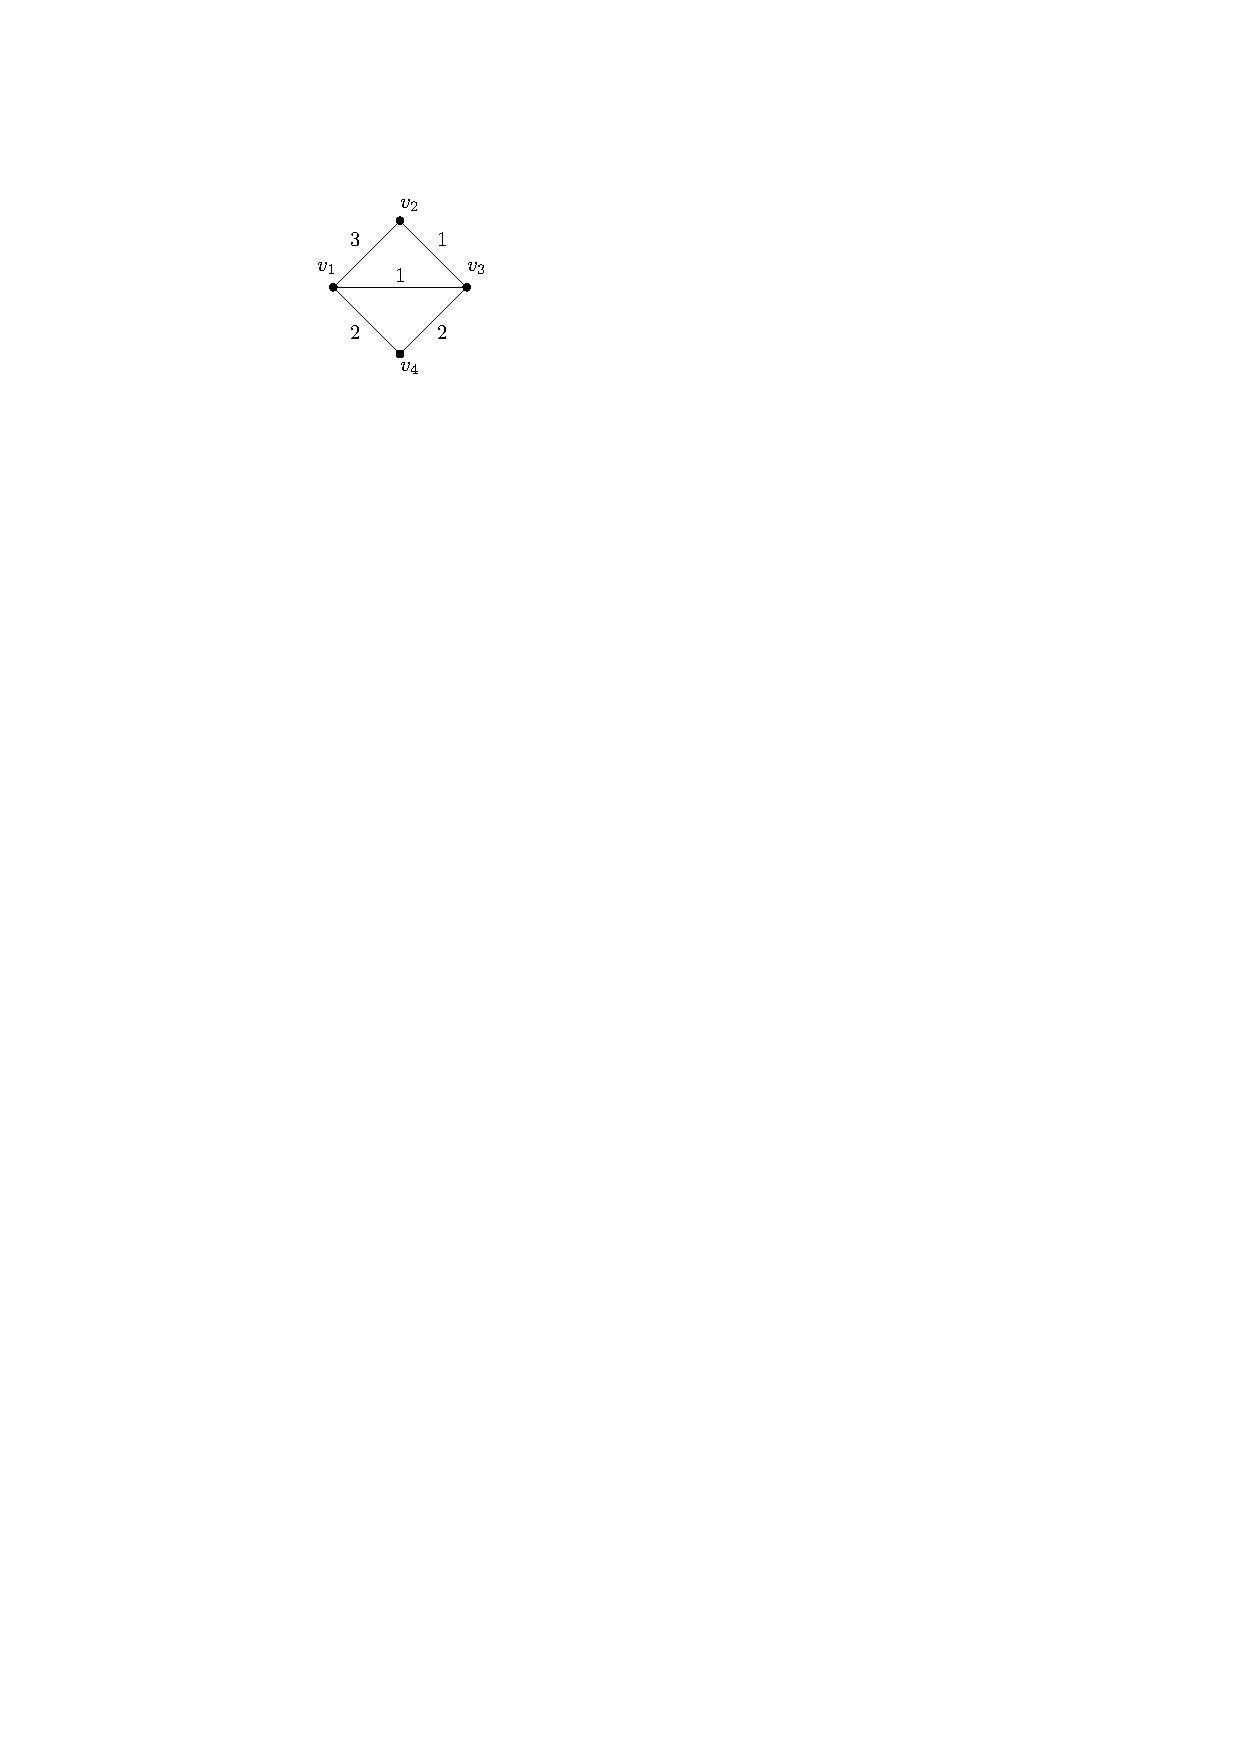
\includegraphics[scale=1]{img/greedy-incorrect}
\caption{Example of a graph, where the Greedy algorithm fails}
\label{fig_greedy_fail}
\end{figure}

\begin{theorem}
(i) The Greedy algorithm is an $(n-1)$-approximation for problem {\act}.
(ii) This is tight in the following sense: There are instances, where the result of the Greedy algorithm is a factor $n/2$ worse than the optimum.
\end{theorem}
\begin{proof}
For the proof of (i), let $(G, w)$ with $G = (V, E)$ be an instance of {\act}, and let $\text{OPT}$ be its optimal solution value. Consider a run of the Greedy-algorithm and let $i$ be the step in which the algorithm stops, because $A' = \emptyset$. We have that $E_i$ is not spanning, hence the graph $(V, E_i)$ has at least two components. Let $C \subseteq V$ be the vertex set of one of these components, consider the edge cut $\delta(C)$ and its weight $w(\delta(C)) := \sum_{e \in \delta(C)}w(e)$. We have that in step $i$, none of the edges of $\delta(C)$ were available, hence they were all chosen at sooner steps than step $i$. Furthermore, in each of the previous steps $j \in \fromto{1}{i-1}$, we have that $|E_j \cap \delta(C)| \leq n-1$, because a spanning tree has $n-1$ edges, hence $|E_j| = n-1$. But this implies that the number of previous steps is at least $i - 1 \geq w(\delta(C)) / (n-1)$. But note that clearly   $\text{OPT} \leq w(\delta(C))$. This proves the claim.

For the proof of (ii), let $G = K_n$ be the complete graph on $n$ vertices. Fix a single vertex $x$, some small rational number $\epsilon > 0$, and consider the following edge weights: If an edge $e$ is adjacent to $x$, we let $w(e) = 1 + \epsilon$, otherwise $w(e) = 1$. The weights can be made integral by multiplication with a large integer. Now the Greedy algorithm returns a schedule of value $1 + \epsilon$. However, it is known that the maximum number of edge-disjoint spanning trees that can be packed into $K_n$ is equal to $\lfloor n/2 \rfloor$ (see \cite{SPTpackingSurvey}). This implies that $\text{OPT} = \lfloor n/2 \rfloor$ in this case, proving the claim.  
\end{proof}
\comment{Can we get rid of factor 1/2 in part (ii)?}


\section{Conclusion}

\begin{itemize}
\item Computational complexity mostly solved: Both problems remain NP-complete if either treewidth or edge weights are bounded by a constant. If both are bounded, $\act$ can be solved in linear time. But we don't know whether $\stact$ can be solved polynomially in this case. 
\item Understanding approximability properties is mostly open. We showed that $\act$ can not be approximated by a factor better than $7/6$ even if $w(e) \in \fromto{1}{6}$. But we don't know whether an analogous result holds for $\stact$. We also were not able to find approximation algorithms for $\act$  with $\bigO(1)$ approximation ratios or any reasonable approximation algorithm for \stact. \textbf{Conjecture:} In the general case, there exists no $\bigO(1)$-approximation algorithm for either {\act} or \stact.
\item FPT results for {\act} could be obtained. FPT results for \stact\ still missing.
\end{itemize}


%\begin{table}
%\begin{tabular}{r|rrrr}
%& $T = \bigO(1) \land \tw = \bigO(1)$ & $l = \bigO(1) \land \tw = \bigO(1)$ & $l = \bigO(1)$ & $\tw = \bigO(1)$\\
%\hline
%$\act$ & $\bigO(n)$ & $\bigO(n)$ & NPC & strongly NPC \\
%$\stact$ & $\bigO(n)$ & ? & NPC & (strongly?) NPC \\
%\end{tabular}
%\caption{Hardness results (? = unknown)}
%\label{table_complexity}
%\end{table}
%
%\begin{table}
%\begin{tabular}{r|rr}
%& lower bound & upper bound \\
%\hline
%$\act$ & 7/6 & ?  \\
%$\stact$ & ? & ? \\
%\end{tabular}
%\caption{Approximation results (? = unknown) \comment{This table not in final paper, only here for ourselves to see what's still open}}
%\end{table}

\subsubsection*{Acknowledgements.}

Stefan Lendl and Lasse Wulf acknowledge the support of the Austrian Science Fund (FWF):
W1230.

%
% ---- Bibliography ----
%
% BibTeX users should specify bibliography style 'splncs04'.
% References will then be sorted and formatted in the correct style.

\bibliographystyle{splncs04}
\bibliography{literature}


\appendix

\section{Connection to job scheduling}
\label{appendix:connection_act_job_scheduling}
A \emph{matroid} is defined as ...
Problem {\act} is related to job scheduling in the following way: Let $G = (V, E)$ be a graph. The \emph{graphic matroid} of $G$ is the set system $\set{F \subseteq E \mid F \text{ is acyclic}}$. A \emph{base} in a matroid is an independent set of maximal cardinality. Hence problem {\act} has the following generalization: Given a ground set $E$, weights $w: E \rightarrow \N$, and some matroid $\mathcal{F} \subseteq 2^E$, find activation times such that for a maximal amount of time, the set of active elements comprises a base of $\mathcal{F}$. Now, let $E$ be a set of jobs, where job $e \in E$ has processing times $w(e)$. For $k \in \N$, the set system $\mathcal{F} = \set{F \subseteq E : |F| = k}$ is a matroid, the so-called the \emph{uniform matroid of rank $k$}. One can now observe that the matroid activation problem for the uniform matroid is exactly the problem of maximizing the minimum machine load time when distributing the jobs onto $k$ machines. In this way, one can see that problem {\act} is a graph-theoretic variant of the problem of maximizing the minimum machine load time.

\section{Proof of \cref{hamilton_cycle_lemma}}

\label{appendix:hamilton_prime}
\hamiltonPrime*

\begin{proof}
It is known that the Hamilton cycle problem is NP-complete for bipartite, 3-regular graphs \cite{hamilton3regularBip}. So let $G = (V, E)$ be a bipartite, 3-regular graph. We construct in polynomial time a graph $H$ and an edge $\set{u,z}$, such that the described propeprties for $(H, \set{u,z})$ hold, and such that $H$ has a Hamilton cycle if and only if $G$ has a Hamilton cycle. If we can show this, we are done.

The reduction is shown in \cref{fig_hamilton_cycle_lemma}. Formally, fix some vertex $x \in V$. Let $G_1$ and $G_2$ be two copies of $G$. For each vertex $v \in V \setminus \set{x}$, take a copy $A_v$ of $K_{4,4}$, remove some edge $\set{u_1, u_2}$ from $A_v$, and add edges $\set{v_1,u_1}$ and $\set{u_2,v_2}$, where $v_i$ is the copy of $v$ in $G_i$, $i = 1,2$. Finally, take two copies $A_x$ and $A'_x$ of $K_{4,4}$, remove an edge $\set{u_1,u_2}$ from $A_x$ and an edge $\set{u'_1,u'_2}$ from $A'_x$, add edges $\set{x_1,u_1}$, $\set{u_2,u'_1}$, $\set{u'_2,x_2}$, and let the special edge be given by $\set{u, z}$ with $u := u_2$, and $z := u'_1$. Clearly, $H$ is bipartite and 4-regular.

Let (iv) be the property that $G$ has a Hamilton cycle. We show that (i) -- (iv) are equivalent, thus proving the theorem. So assume (i) holds. It is easy to see that any Hamilton cyle in $H$ uses $\set{u,z}$, so (ii) holds. Assume (ii) holds, (iii) follows immediately. Assume (iii) holds, i.e.\ there is a Hamilton path $(w_1, \dots, w_n)$ starting at $u$. Note that if $w_2 = z$, then $w_n$ is in $A_x$. On the other hand, if $w_2$ is in $A_x$, then $w_n$ is in $A'_x$. In both cases, we can slightly modify $P$ to obtain a Hamilton cycle. Therefore, (i) holds. Finally, we show that (i) and (iv) are equivalent. If $G$ has a Hamilton cycle, we can modify it to obtain a Hamilton cycle of $H$, by switching between $G_1$ and $G_2$ after every edge of the original Hamilton cycle and inserting a Hamilton path through the copies of $K_{4,4}$ (note that $G$ has an even number of vertices, as it is 3-regular). On the other hand, if $H$ has a Hamilton cycle, it necessarily switches between $G_1$ and $G_2$ after every of its edges in $G_1$ or $G_2$, so $G$ has a Hamilton cycle.
\end{proof}
\begin{figure}[htpb]
\centering
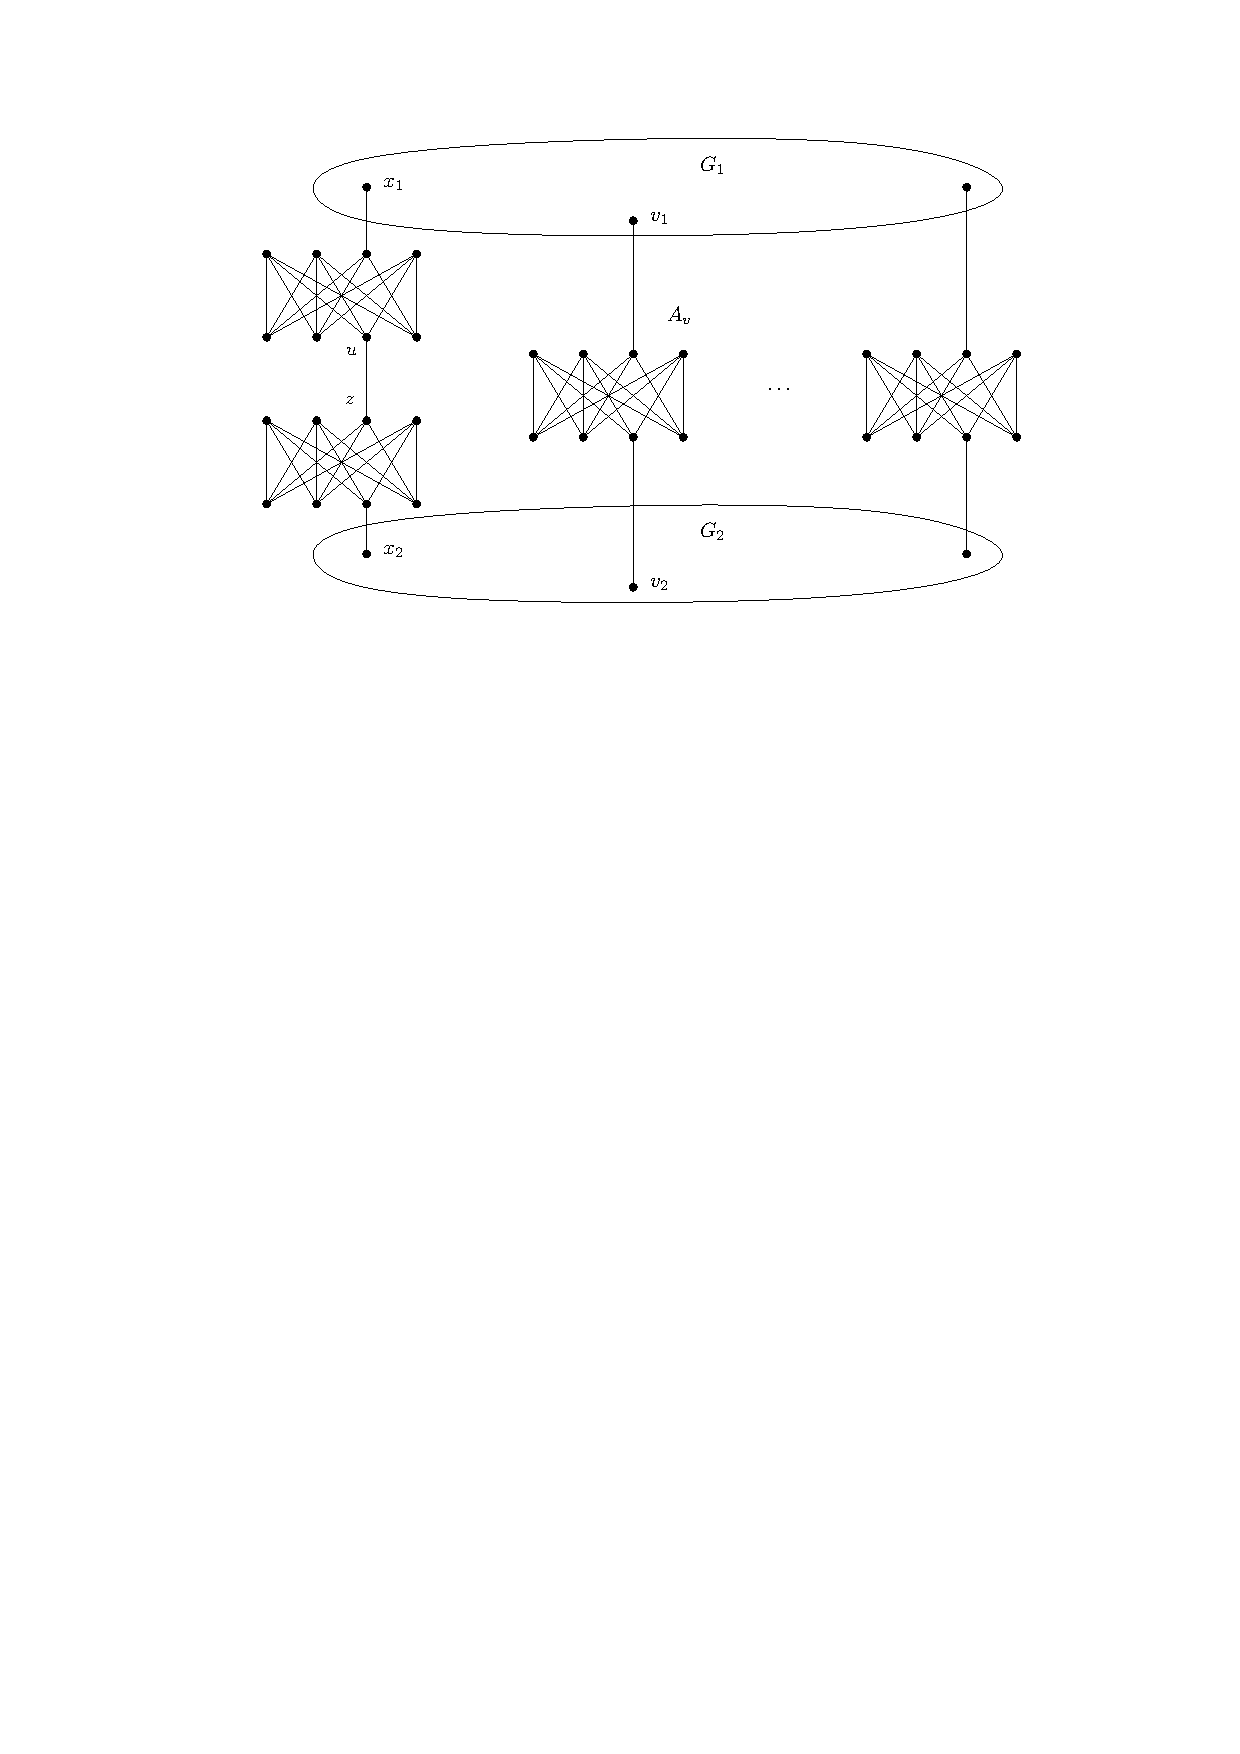
\includegraphics[scale=1]{img/hamilton-prime}
\caption{Construction used in the proof of \cref{hamilton_cycle_lemma}.}
\label{fig_hamilton_cycle_lemma}
\end{figure}

\end{document}